\section{C. 즐거운 XOR}

\begin{frame} % No title at first slide
    \sectiontitle{C}{즐거운 XOR}
    \sectionmeta{
        \texttt{combinatorics}\\
        출제진 의도 -- \textbf{\color{acsilver}Easy}
    }
    \begin{itemize}
        \item 출제자: \texttt{riroan}
    \end{itemize}
\end{frame}

\begin{frame}{\textbf{C}. 즐거운 XOR}
    \begin{figure}[h!]
        \centering
        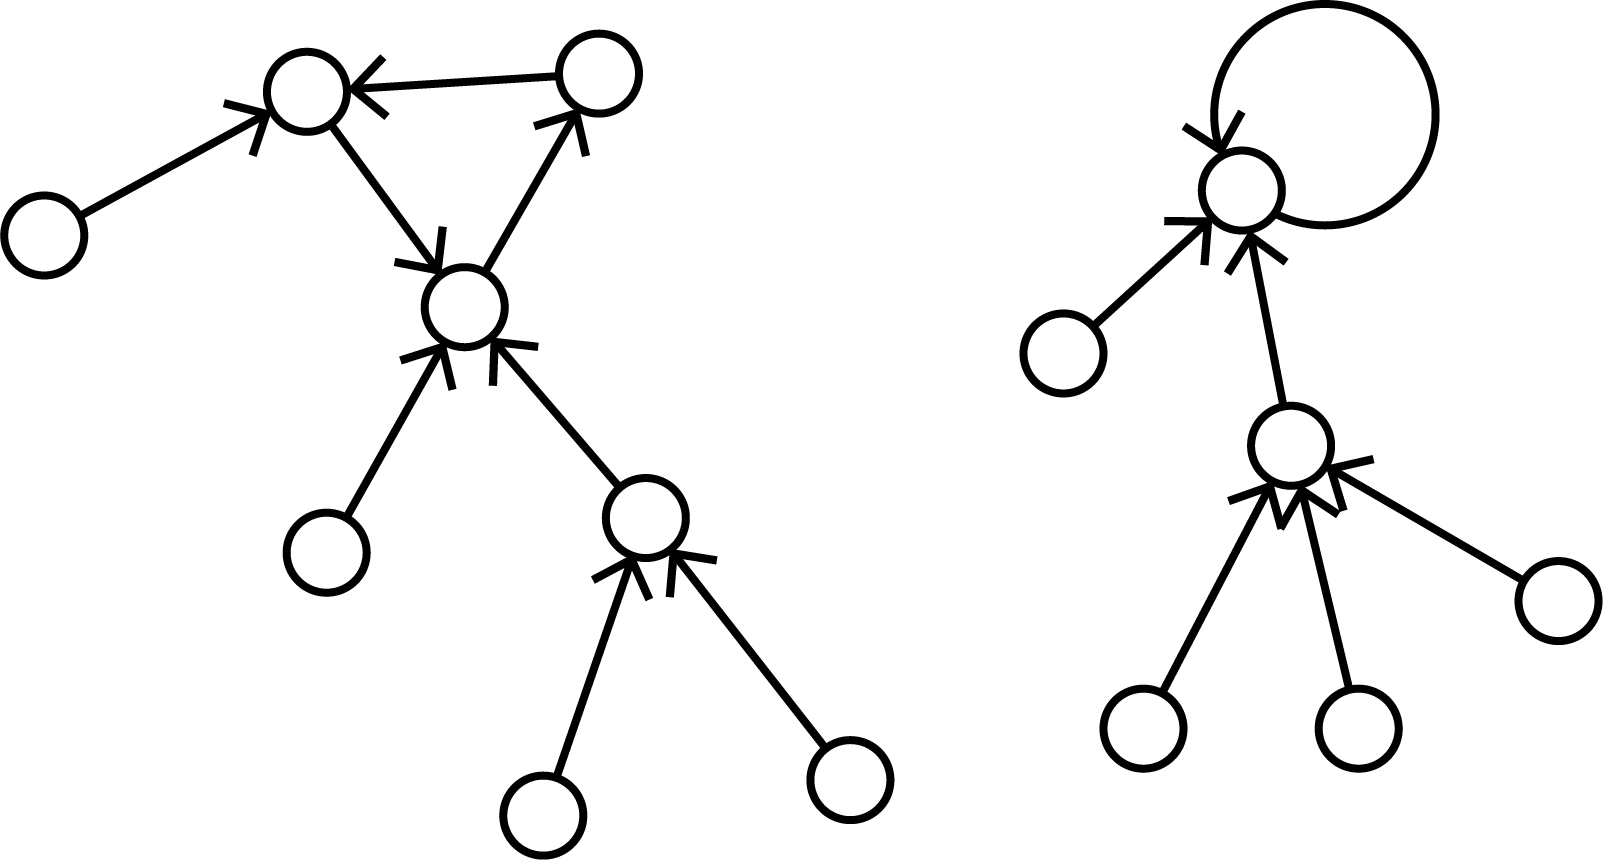
\includegraphics[width=0.5\linewidth]{../images/function-restore/fx-1n.png}
    \end{figure}
    \begin{itemize}
        \item 함수 그래프는 각 컴포넌트가 하나의 사이클에 연결된 트리들로 이루어져 있습니다.
        \item 자기보다 더 적은 수의 정점에 도달할 수 있는 정점이 있다면 트리에 속하고, 그렇지 않으면 사이클에 속하는 정점입니다.
    \end{itemize}
\end{frame}